\chapter{Background and Related Work}
% In this chapter, we detail the background and prior research that underpins the work described in later chapters. Further, we include an explanation of the theoretical concepts, both reinforcement learning and graph neural networks, which we have used extensively in this work.

\section{Introduction to Deep Learning Models}
This section discusses the way in which machine learning models are represented for efficient execution on physical hardware devices. First, we discuss how the mapping of tensor operations to computation graphs is performed followed by an overview of recent approaches that optimise computation graphs to minimise execution time.

Over the past decade, there has been a rapid development of various deep learning architectures that aim to solve a specific task. Common examples include convolutional networks (popularised by AlexNet then ResNets, etc), transformer networks that have seen use in the modelling and generation of language. Recurrent networks that have shown to excel at learning long and short trends in data.

Importantly, the fundamental building blocks of the networks have largely remained unchanged.  As the networks become more complex, it becomes untenable to manually optimise the networks to reduce the execution time on hardware. Therefore, there is extensive work in ways to both automatically optimise the models, or, alternatively apply a set of hand-crafted optimisations.

Computation graphs are a way to graphically represent both the individual tensor operations in a model, and the connections (or data-flow) along the edges between nodes in the graph. Figure \ref{fig:bg:perceptron} shows how the expression, $y = \texttt{ReLU}(\mathbf{w} \cdot \mathbf{x} + b)$, can be represented graphically in a computation graph.

\begin{figure}[ht]
  \centering
  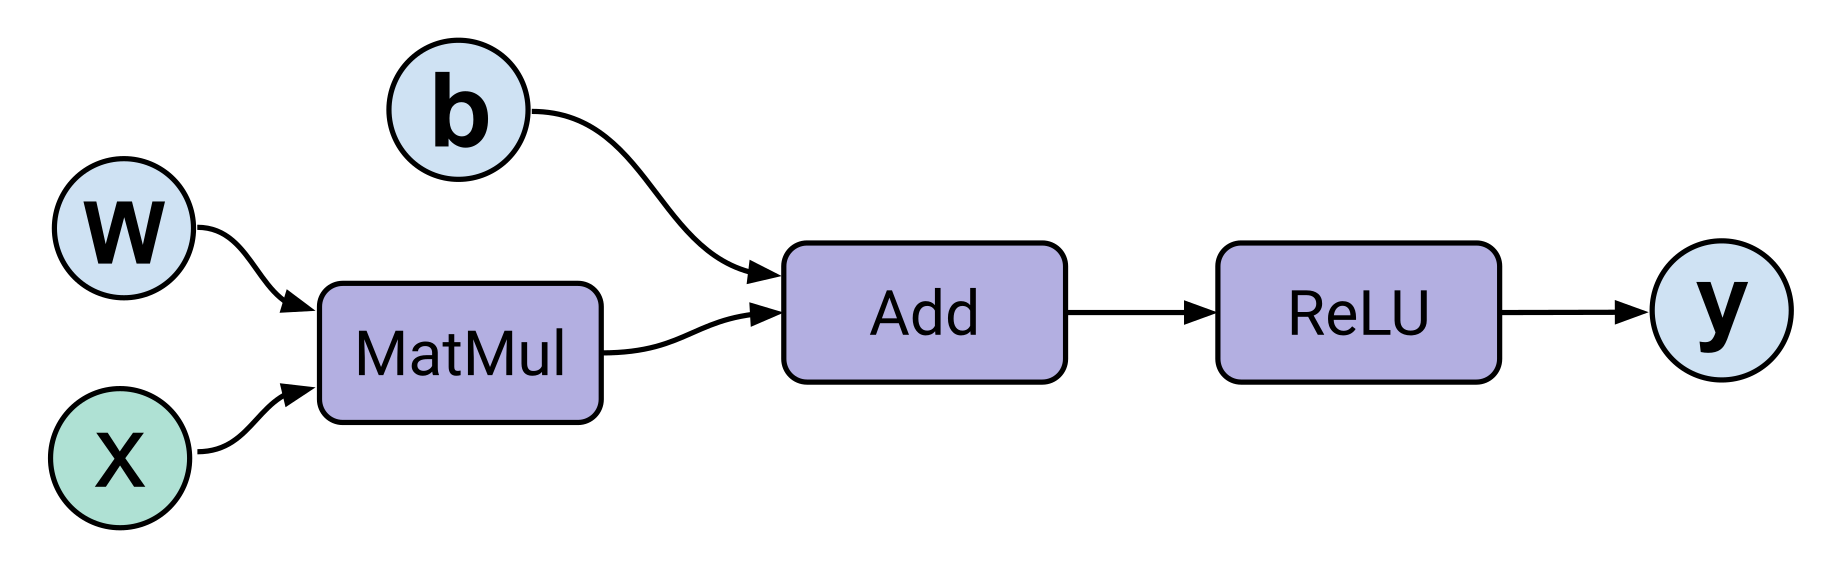
\includegraphics[width=0.75\columnwidth]{sections/2background/images/bitmap}
  \caption[Single perceptron as a dataflow (computation) graph]{The operations shown in purple are the nodes of the computation graph which take an arbitraty number of inputs, performs a computation at the node and produces an output. The blue nodes represent the input nodes for tensors. The directed edges show the flow of tensors through the graph.}
  \label{fig:bg:perceptron}
\end{figure}

Similarly, the whole model can be converted into a stateful dataflow graph in this manner. By using a stateful dataflow (or computation) graph, we can use any optimisation technique for backpropagation of the model loss though the graph [TODO rewrite last sentence]. We consider two key benefits of this representation. First, we can execute the model on any hardware device as the models have a single, uniform representation. Secondly, it allows for pre-execution optimisations based on the host device, for example, we may perform different optimisations for executing on a GPU compared to a TPU.

\subsection{Current approaches to optimising deep learning models}

Due to the prevalence and importance of machine learning, especially deep networks, there is a focus on finding ways decrease the inference runtime and by extension, increasing the model throughput. All major frameworks such as Tensorflow \cite{tensorflow2015-whitepaper}, PyTorch \cite{}, MXNet, and Caffe have some level of support for performing pre-execution optimisations. However, the process of performing such optimisations is often time-consuming and cannot be completed in real-time. Rather, it is to use a deep learning optimisation library such as cuDNN \cite{chetlur2014cudnn}.

%common machine learning framework is designed to greedily apply a set of pre-defined substitutions to an input graph in an attempt to optimise the graph. Tensorflow made use of low-level libraries such as cuBLAS \cite{cublas2008} for optimised matrix operations and cuDNN \cite{chetlur2014cudnn} for convolutional kernels. Furthermore, Tensorflow also contains a set of 155 substitutions that are implemented in 53,000 lines of code; to complicate matters, new operators are continuously proposed, such as grouped or transposed convolutions, all of which leads to a large amount of engineering effort required to maintain the library.

%TensorRT \cite{tensorrt2017} provides a high-performance SDK to optimise the inference of models via a combination of techniques such as layout and tensor fusion, auto-tuning kernels, and multi-stream execution. The SDK acts as both the optimisation and execution engine that lies between the ML framework and physical hardware. Importantly, it is not involved during the training process, rather, it assumes for the best possible performance that the developer 
TVM

Metaflow and TASO

\section{Reinforcement Learning}
Reinforcement learning (RL) is a sub-field in machine learning, broadly, it aims to compute a control policy such that an agent can maximise its cumulative reward from the environment. It has powerful applications in environments where a model that describes the semantics of the system are not available and the agent must itself discover the optimal strategy via a reward signal. Formally, RL is a class of learning problem that can be framed as a Markov decision processes (MDP) when the MDP that describes the system is not known \cite{bellman1957}; they are represented as a tuple $\langle \mathcal{S}, \mathcal{A}, \mathcal{P}_a, \mathcal{R}_a \rangle$ where:

\begin{itemize}
  \item $\mathcal{S}$, is a finite set of states
  \item $\mathcal{A}$, is a finite set of actions
  \item $\mathcal{P}_a$, is the state transition probability that an action $a$ in state $s_t$ leads to a state $s'_{t+1}$
  \item $\mathcal{R}_a$, is the reward from the environment after taking an action $a$ between state $s_t$ and $s'_{t+1}$
\end{itemize}

% TODO: add citations
We aim to compute a policy, denoted by $\pi$, that when given a state $s \in \mathcal{S}$, returns an action $a \in \mathcal{A}$ with the optimisation objective being to find a control policy $\pi^*$ that maximises the \textit{expected reward} from the environment defined by \ref{equ:expec-rew}. Notably, we can control the `far-sightedness' of the policy by tuning the discount factor $\gamma \in [0, 1]$. As $\gamma$ tends to 1, the policy considers the rewards further in the future but with a lower weight as the distant expected reward may be an imperfect prediction.

\begin{equation}
  \label{equ:expec-rew}
  \pi^* = \argmax_\pi~\mathbb{E} \left[ \sum^\infty_{t=0} \gamma^t~\mathcal{R}_t \right]
\end{equation}

Recent success with reinforcement learning can be attributed, in part, to the success of modern deep learning function approximators, such as neural networks, which make learning the solutions far more efficient in practise.

has been successfully applied to a wide range of fields, for example, robotic control tasks \cite{openai2019solving}, datacenter power management, device placement, and, playing both perfect and imperfect information games to a super-human level. Reinforcement learning excels when applied to environments in which actions may have long-term, inter-connected dependencies that are difficult to learn or model with traditional machine learning techniques.

In the following sections we discuss the two key paradigms that exist in reinforcement learning and the current research in both areas and the application to systems tasks.

\subsection{Model-Free and Model-Based RL}


\section{Graph Neural Networks}